\begin{table}[p]
   \centering
   \scriptsize
   \renewcommand{\arraystretch}{1.1}
   \begin{tabular}{@{}>{\centering\arraybackslash}m{0.413\textwidth}>{\centering\arraybackslash}m{0.414\textwidth}>{\centering\arraybackslash}m{0.083\textwidth}@{}}
      \hline
      \multicolumn{3}{@{}c@{}}{%
         \begin{tabular}{@{}>{\centering\arraybackslash}m{\dimexpr0.455\textwidth+\tabcolsep\relax}>{\centering\arraybackslash}m{\dimexpr0.455\textwidth+\tabcolsep\relax}@{}}
            $T_1$ & Matriz de adyacencia \\
            \hline
            \noalign{\vspace{6pt}}
            \rule{0pt}{0pt}$\vcenter{\hbox{\resizebox{0.32\textwidth}{!}{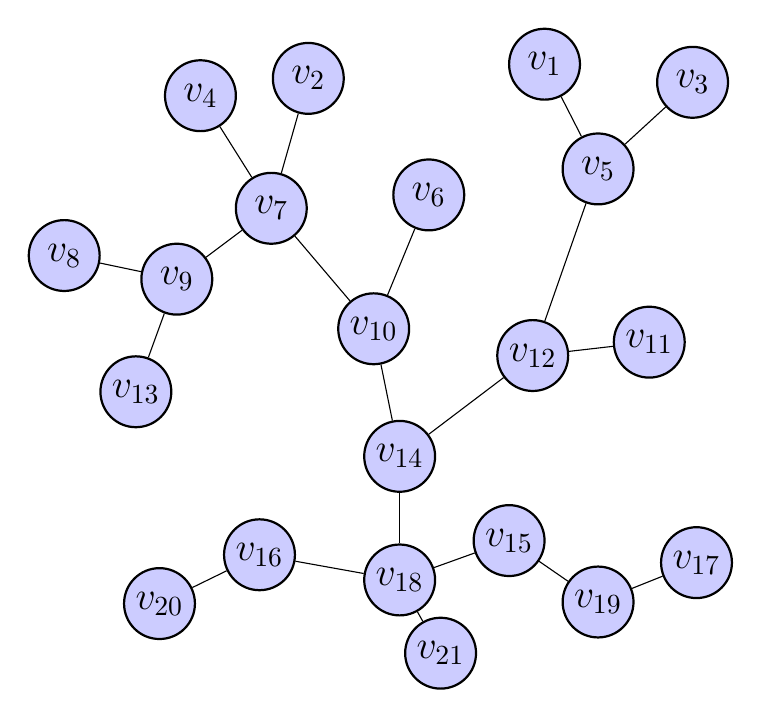
\begin{tikzpicture}[
  scale=1,
  vnode/.style={circle, fill=blue!20, draw=black, thick, minimum size=9mm, inner sep=0pt, font=\Large}
]
  % Vértices
  \node[vnode] (v1) at (7.12, 7.78) {$v_1$};
  \node[vnode] (v2) at (4.12, 7.60) {$v_2$};
  \node[vnode] (v3) at (9.00, 7.55) {$v_3$};
  \node[vnode] (v4) at (2.75, 7.38) {$v_4$};
  \node[vnode] (v5) at (7.80, 6.45) {$v_5$};
  \node[vnode] (v6) at (5.65, 6.12) {$v_6$};
  \node[vnode] (v7) at (3.65, 5.95) {$v_7$};
  \node[vnode] (v8) at (1.02, 5.35) {$v_8$};
  \node[vnode] (v9) at (2.45, 5.05) {$v_9$};
  \node[vnode] (v10) at (4.95, 4.42) {$v_{10}$};
  \node[vnode] (v11) at (8.45, 4.25) {$v_{11}$};
  \node[vnode] (v12) at (6.97, 4.08) {$v_{12}$};
  \node[vnode] (v13) at (1.93, 3.62) {$v_{13}$};
  \node[vnode] (v14) at (5.28, 2.80) {$v_{14}$};
  \node[vnode] (v15) at (6.67, 1.73) {$v_{15}$};
  \node[vnode] (v16) at (3.50, 1.55) {$v_{16}$};
  \node[vnode] (v17) at (9.05, 1.45) {$v_{17}$};
  \node[vnode] (v18) at (5.28, 1.23) {$v_{18}$};
  \node[vnode] (v19) at (7.80, 0.95) {$v_{19}$};
  \node[vnode] (v20) at (2.23, 0.93) {$v_{20}$};
  \node[vnode] (v21) at (5.80, 0.30) {$v_{21}$};

  % Aristas
  \foreach \from/\to in {v1/v5, v2/v7, v3/v5, v4/v7, v5/v12, v6/v10, v7/v9,
                         v7/v10, v8/v9, v9/v13, v10/v14, v11/v12, v12/v14, v14/v18,
                         v15/v18, v15/v19, v16/v18, v16/v20, v17/v19, v18/v21}
    \draw (\from) -- (\to);
\end{tikzpicture}
}}}$
            &
            $\vcenter{\hbox{\tiny$\setcounter{MaxMatrixCols}{21}\setlength{\arraycolsep}{1.6pt}\renewcommand{\arraystretch}{0.9}\begin{pmatrix}
         0 & 0 & 0 & 0 & 1 & 0 & 0 & 0 & 0 & 0 & 0 & 0 & 0 & 0 & 0 & 0 & 0 & 0 & 0 & 0 & 0 \\
         0 & 0 & 0 & 0 & 0 & 0 & 1 & 0 & 0 & 0 & 0 & 0 & 0 & 0 & 0 & 0 & 0 & 0 & 0 & 0 & 0 \\
         0 & 0 & 0 & 0 & 1 & 0 & 0 & 0 & 0 & 0 & 0 & 0 & 0 & 0 & 0 & 0 & 0 & 0 & 0 & 0 & 0 \\
         0 & 0 & 0 & 0 & 0 & 0 & 1 & 0 & 0 & 0 & 0 & 0 & 0 & 0 & 0 & 0 & 0 & 0 & 0 & 0 & 0 \\
         1 & 0 & 1 & 0 & 0 & 0 & 0 & 0 & 0 & 0 & 0 & 1 & 0 & 0 & 0 & 0 & 0 & 0 & 0 & 0 & 0 \\
         0 & 0 & 0 & 0 & 0 & 0 & 0 & 0 & 0 & 1 & 0 & 0 & 0 & 0 & 0 & 0 & 0 & 0 & 0 & 0 & 0 \\
         0 & 1 & 0 & 1 & 0 & 0 & 0 & 0 & 1 & 1 & 0 & 0 & 0 & 0 & 0 & 0 & 0 & 0 & 0 & 0 & 0 \\
         0 & 0 & 0 & 0 & 0 & 0 & 0 & 0 & 1 & 0 & 0 & 0 & 0 & 0 & 0 & 0 & 0 & 0 & 0 & 0 & 0 \\
         0 & 0 & 0 & 0 & 0 & 0 & 1 & 1 & 0 & 0 & 0 & 0 & 1 & 0 & 0 & 0 & 0 & 0 & 0 & 0 & 0 \\
         0 & 0 & 0 & 0 & 0 & 1 & 1 & 0 & 0 & 0 & 0 & 0 & 0 & 1 & 0 & 0 & 0 & 0 & 0 & 0 & 0 \\
         0 & 0 & 0 & 0 & 0 & 0 & 0 & 0 & 0 & 0 & 0 & 1 & 0 & 0 & 0 & 0 & 0 & 0 & 0 & 0 & 0 \\
         0 & 0 & 0 & 0 & 1 & 0 & 0 & 0 & 0 & 0 & 1 & 0 & 0 & 1 & 0 & 0 & 0 & 0 & 0 & 0 & 0 \\
         0 & 0 & 0 & 0 & 0 & 0 & 0 & 0 & 1 & 0 & 0 & 0 & 0 & 0 & 0 & 0 & 0 & 0 & 0 & 0 & 0 \\
         0 & 0 & 0 & 0 & 0 & 0 & 0 & 0 & 0 & 1 & 0 & 1 & 0 & 0 & 0 & 0 & 0 & 1 & 0 & 0 & 0 \\
         0 & 0 & 0 & 0 & 0 & 0 & 0 & 0 & 0 & 0 & 0 & 0 & 0 & 0 & 0 & 0 & 0 & 1 & 1 & 0 & 0 \\
         0 & 0 & 0 & 0 & 0 & 0 & 0 & 0 & 0 & 0 & 0 & 0 & 0 & 0 & 0 & 0 & 0 & 1 & 0 & 1 & 0 \\
         0 & 0 & 0 & 0 & 0 & 0 & 0 & 0 & 0 & 0 & 0 & 0 & 0 & 0 & 0 & 0 & 0 & 0 & 1 & 0 & 0 \\
         0 & 0 & 0 & 0 & 0 & 0 & 0 & 0 & 0 & 0 & 0 & 0 & 0 & 1 & 1 & 1 & 0 & 0 & 0 & 0 & 1 \\
         0 & 0 & 0 & 0 & 0 & 0 & 0 & 0 & 0 & 0 & 0 & 0 & 0 & 0 & 1 & 0 & 1 & 0 & 0 & 0 & 0 \\
         0 & 0 & 0 & 0 & 0 & 0 & 0 & 0 & 0 & 0 & 0 & 0 & 0 & 0 & 0 & 1 & 0 & 0 & 0 & 0 & 0 \\
         0 & 0 & 0 & 0 & 0 & 0 & 0 & 0 & 0 & 0 & 0 & 0 & 0 & 0 & 0 & 0 & 0 & 1 & 0 & 0 & 0
      \end{pmatrix}$}}$ \\
            \noalign{\vspace{6pt}}
         \end{tabular}%
      } \\
      \hline
      \multicolumn{3}{c}{\textbf{Topología de adyacencia}} \\
      \hline
      Abiertos subbásicos & Vecindades mínimas & Topología \\
      \hline
         \vspace{3pt}\begin{tabular}{@{}l@{\hspace{0.4em}}l@{}}
            ${A_{v_1}=\{v_5\}}$ & ${A_{v_{12}}=\{v_5,v_{11},v_{14}\}}$ \\
            ${A_{v_2}=\{v_7\}}$ & ${A_{v_{13}}=\{v_9\}}$ \\
            ${A_{v_3}=\{v_5\}}$ & ${A_{v_{14}}=\{v_{10},v_{12},v_{18}\}}$ \\
            ${A_{v_4}=\{v_7\}}$ & ${A_{v_{15}}=\{v_{18},v_{19}\}}$ \\
            ${A_{v_5}=\{v_1,v_3,v_{12}\}}$ & ${A_{v_{16}}=\{v_{18},v_{20}\}}$ \\
            ${A_{v_6}=\{v_{10}\}}$ & ${A_{v_{17}}=\{v_{19}\}}$ \\
            ${A_{v_7}=\{v_2,v_4,v_9,v_{10}\}}$ & ${A_{v_{18}}=\{v_{14},v_{15},v_{16},v_{21}\}}$ \\
            ${A_{v_8}=\{v_9\}}$ & ${A_{v_{19}}=\{v_{15},v_{17}\}}$ \\
            ${A_{v_9}=\{v_7,v_8,v_{13}\}}$ & ${A_{v_{20}}=\{v_{16}\}}$ \\
            ${A_{v_{10}}=\{v_6,v_7,v_{14}\}}$ & ${A_{v_{21}}=\{v_{18}\}}$ \\
            ${A_{v_{11}}=\{v_{12}\}}$ &  \\
         \end{tabular}\vspace{3pt}
      &
         \vspace{3pt}\begin{tabular}{@{}l@{\hspace{0.4em}}l@{}}
            ${U_{v_1}=\{v_1,v_3,v_{12}\}}$ & ${U_{v_{12}}=\{v_{12}\}}$ \\
            ${U_{v_2}=\{v_2,v_4,v_9,v_{10}\}}$ & ${U_{v_{13}}=\{v_7,v_8,v_{13}\}}$ \\
            ${U_{v_3}=\{v_1,v_3,v_{12}\}}$ & ${U_{v_{14}}=\{v_{14}\}}$ \\
            ${U_{v_4}=\{v_2,v_4,v_9,v_{10}\}}$ & ${U_{v_{15}}=\{v_{15}\}}$ \\
            ${U_{v_5}=\{v_5\}}$ & ${U_{v_{16}}=\{v_{16}\}}$ \\
            ${U_{v_6}=\{v_6,v_7,v_{14}\}}$ & ${U_{v_{17}}=\{v_{15},v_{17}\}}$ \\
            ${U_{v_7}=\{v_7\}}$ & ${U_{v_{18}}=\{v_{18}\}}$ \\
            ${U_{v_8}=\{v_7,v_8,v_{13}\}}$ & ${U_{v_{19}}=\{v_{19}\}}$ \\
            ${U_{v_9}=\{v_9\}}$ & ${U_{v_{20}}=\{v_{18},v_{20}\}}$ \\
            ${U_{v_{10}}=\{v_{10}\}}$ & ${U_{v_{21}}=\{v_{14},v_{15},v_{16},v_{21}\}}$ \\
            ${U_{v_{11}}=\{v_5,v_{11},v_{14}\}}$ &  \\
         \end{tabular}\vspace{3pt}
      &
         No discreta, con 14040 abiertos \\
      \hline
      \multicolumn{3}{c}{\textbf{Topología de incidencia}} \\
      \hline
      Abiertos subbásicos & Vecindades mínimas & Topología \\
      \hline
         \vspace{3pt}\begin{tabular}{@{}l@{\hspace{0.4em}}l@{}}
            ${e_{1}=\{v_1,v_5\}}$ & ${e_{11}=\{v_{10},v_{14}\}}$ \\
            ${e_{2}=\{v_2,v_7\}}$ & ${e_{12}=\{v_{11},v_{12}\}}$ \\
            ${e_{3}=\{v_3,v_5\}}$ & ${e_{13}=\{v_{12},v_{14}\}}$ \\
            ${e_{4}=\{v_4,v_7\}}$ & ${e_{14}=\{v_{14},v_{18}\}}$ \\
            ${e_{5}=\{v_5,v_{12}\}}$ & ${e_{15}=\{v_{15},v_{18}\}}$ \\
            ${e_{6}=\{v_6,v_{10}\}}$ & ${e_{16}=\{v_{15},v_{19}\}}$ \\
            ${e_{7}=\{v_7,v_9\}}$ & ${e_{17}=\{v_{16},v_{18}\}}$ \\
            ${e_{8}=\{v_7,v_{10}\}}$ & ${e_{18}=\{v_{16},v_{20}\}}$ \\
            ${e_{9}=\{v_8,v_9\}}$ & ${e_{19}=\{v_{17},v_{19}\}}$ \\
            ${e_{10}=\{v_9,v_{13}\}}$ & ${e_{20}=\{v_{18},v_{21}\}}$ \\
         \end{tabular}\vspace{3pt}
      &
         \vspace{3pt}\begin{tabular}{@{}l@{\hspace{0.4em}}l@{}}
            ${U_{v_1}=\{v_1,v_5\}}$ & ${U_{v_{12}}=\{v_{12}\}}$ \\
            ${U_{v_2}=\{v_2,v_7\}}$ & ${U_{v_{13}}=\{v_9,v_{13}\}}$ \\
            ${U_{v_3}=\{v_3,v_5\}}$ & ${U_{v_{14}}=\{v_{14}\}}$ \\
            ${U_{v_4}=\{v_4,v_7\}}$ & ${U_{v_{15}}=\{v_{15}\}}$ \\
            ${U_{v_5}=\{v_5\}}$ & ${U_{v_{16}}=\{v_{16}\}}$ \\
            ${U_{v_6}=\{v_6,v_{10}\}}$ & ${U_{v_{17}}=\{v_{17},v_{19}\}}$ \\
            ${U_{v_7}=\{v_7\}}$ & ${U_{v_{18}}=\{v_{18}\}}$ \\
            ${U_{v_8}=\{v_8,v_9\}}$ & ${U_{v_{19}}=\{v_{19}\}}$ \\
            ${U_{v_9}=\{v_9\}}$ & ${U_{v_{20}}=\{v_{16},v_{20}\}}$ \\
            ${U_{v_{10}}=\{v_{10}\}}$ & ${U_{v_{21}}=\{v_{18},v_{21}\}}$ \\
            ${U_{v_{11}}=\{v_{11},v_{12}\}}$ &  \\
         \end{tabular}\vspace{3pt}
      &
         No discreta, con 121500 abiertos \\
      \hline
   \end{tabular}
   \caption{Topologías de adyacencia e incidencia de $T_1$}
   \label{tab:topologias_T_1}
\end{table}
